\section{Six Sigma Approaches}
% Fundamentals and Handbook for process management
The first set of analysation and optimization techniques discussed in this chapter originate from the Six Sigma initiative. The name Six Sigma originates from the interval of $6\sigma$ in the normal distribution that indicates the aimed success rate of $99.99966\%$ \cite{siha2008business}\cite{vivekananthamoorthy2011lean} . A representation of the statistical meaning can be see in figure \ref{fig:six-sigma}. Apart from the goal to decrease the error rate, $6\sigma$ is also an methodology for systematically improving process quality \cite{tennant2017six}.

\begin{figure}[H]
		\centering
		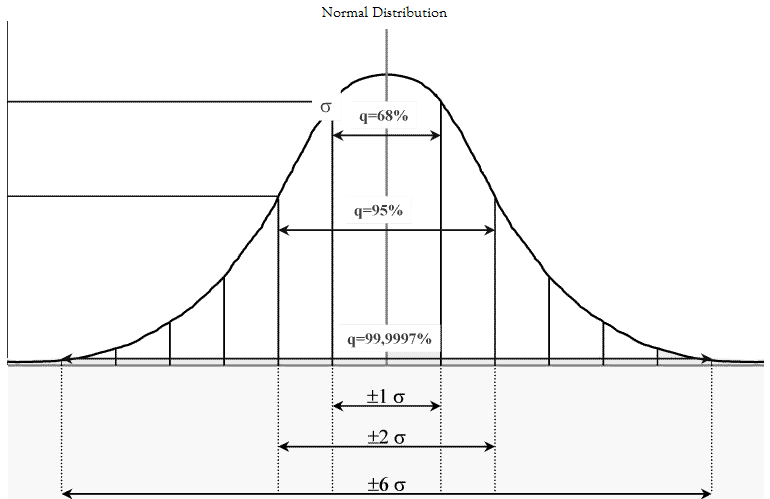
\includegraphics[width=0.7\columnwidth]{graphics/six-sigma}
		\caption{The standard normal distribution showing the $6\sigma$ interval (graphic from \cite{vivekananthamoorthy2011lean})} 
		\label{fig:six-sigma} 
\end{figure}

Applied in the context of (executable) business processes, Six Sigma provides a set of methods to identify and eliminate inefficient or needless steps in a process \cite{vom2014handbook}. While countless tools are available as part of Six Sigma, the two main methodologies applied in these tools are \gls{DMAIC}, used for improving existing processes, and \gls{DMADV}, used when creating new processes \cite{selvi2014six} .


In the following, a few selected Six Sigma methods are described that apply the \textbf{DMAIC} and  \textbf{DMADV} approach, these being:  
\begin{itemize}
	\item SIPOC Analysis
	\item Check Sheets
	\item Cause and Effect Diagram
	\item Root Cause Analysis
	\item Quality Function Deployment (QFD)
\end{itemize}

\subsection{SIPOC Analysis}
The SIPOC analysis is a tool used in the \textbf{Define} phase of \gls{DMAIC} and \gls{DMADV} and should provide more detailed information about each process step than the \gls{bpmn} model  \cite{vom2014handbook}. 

The outcome of a SIPOC analysis is a table, containing the following information for each task in the process \cite{toutenburg2008six}: 
\begin{itemize}
	\item \textbf{S}upplier: provides the input for this task and influence the output the supplier can be internal or external. 
	\item \textbf{I}nput: Resources, data or material needed for this task provided by the suppliers. 
	\item \textbf{P}rocess: the series of actions taken in this task. This can also be a subprocess. 
	\item \textbf{O}utput: represent the result of this process task and provide value for the customer
	\item \textbf{C}ustomer: the customer that benefits from the output of this task (can be external or internal of the organization)
\end{itemize}



\subsection{Check Sheets}

\subsection{Pareto Analysis}

\subsection{Cause and Effect Diagram}

\subsection{Root Cause Analysis}

\subsection{Quality Function Deployment (QFD)}

\section{Other Qualitative Measures}

\subsection{Value Added Analysis (VAA)}

\section{Quantitative Analysis}
% Fundamentals chapter 7
\subsection{Performance Measures}
\subsection{Flow Analysis}
\subsection{Queues}
\subsection{Simulation}

\section{Benchmarking Processes}

%H. Harrington - Business Process Improvement chapter 9 